\documentclass{ijsra}
\def\IJSRAidentifier{\currfilebase}
\def\shorttitle{Undergraduate Archaeological Skills Development in Western Autralia}
\def\maintitle{Testing a student driven, non-academic model for undergraduate archaeological skills development in Western Australia}
\def\shortauthor{Jane Fyfe, Sean Winter, Ashleigh Murszewski}
\def\authormail{jane.fyfe@graduate.uwa.edu.au}
%\def\affiliation{1Archaeology M257, University of Western Australia, 35 Stirling Highway, Crawley, Western Australia 6009}
%\def\affiliation{2Australian Archaeomagnetism Laboratory, Department of Archaeology, Faculty of Humanities and Social Sciences, La Trobe University, Melbourne Campus, Bundoora, VIC 3086, Australia}
\def\thanknote{Jane Fyfe is currently completing a PhD in archaeology at the University of Western Australia, and working in Aboriginal Health Training. She has many research interests, including the intersection of historical and Indigenous archaeologies, the role of rock art in all its forms (from prehistoric pigment and engravings to contemporary graffiti) in identity formation and resistance. Jane is also interested in exploring the stories and archaeologies of the unseen and unheard through historical and contemporary archaeology. She is passionate about teaching and sharing archaeology with university students, community volunteers and enthusiasts, especially its practical application and interpretation. She has published in journals her work on historical inscriptions in the Torres Strait and rock art in northern Australia, as well as her PhD research in the southern Kimberley, Western Australia and presented her research at Conferences in the USA and Australia.
	
Sean Winter is an early career researcher currently working in Western Australia. He has diverse research interests with a primary concentration on historical archaeology in Australia. He also has secondary interests in the archaeology of the Greco-Roman period in Egypt; in the archaeology of World War II; in methodological issues related to excavation and stratigraphy, particularly related to urban sites and buildings archaeology; in issues related to teaching and learning in archaeology; and in heritage issues related to convict sites. He has published in numerous journals and will shortly be releasing a book on the convict system in Western Australia.

Ashleigh Murszewski is a developing geoarchaeologist working on various deposits within Western Australia and Southern Africa. With a dual qualification in geology and archaeology, she has pursued an interdisciplinary specialty focusing on understanding geomorphological context of archaeological and palaeoanthropological sites. Current research projects include; local sedimentology of alluvial and karst sequences (inc. micromorphological and sedimentological applications) and, regional studies of palaeocave formation and survival. She has published and presented in Australian journals and conferences on her research in Western Australia, and will commence a PhD at La Trobe University, Melbourne, Victoria in 2016.}
\def\keywords{Community, pedagogy, students, skills development, ethics, research}
%\def\keywordname{}
\begin{filecontents}{\IJSRAidentifier.bib}
@ARTICLE {aitchison2004,
author  = "Ken Aitchison",
title   = "Supply, demand and a failure of understanding: addressing the culture clash between archaeologists' expectations for training and employment in 'academia' versus 'practice'",
journaltitle = "World Archaeology",
year    = "2004",
volume  = "36",
number  = "2",
pages   = "203--219"
}


@MANUAL {AAA2004,
title  = "Code of Ethics",
author = "Australian Archaeological Association Inc.",
year   = "2004"
}


@MANUAL {aacai,
title        = "Code of Ethics",
author       = "AACAI",
organization = "Australian Association of Consulting Archaeologists",
}


@BOOK {beck2008,
editor    = "Beck, W.",
title     = "By Degrees. Benchmarking archaeology degrees in Australian Universities",
publisher = "Teaching and Learning Centre, University of New England",
year      = "2008",
location   = "Armidale, NSW"
}


@ARTICLE {beck2005,
author  = "Beck, W. and Balme, J.",
title   = "Benchmarking for archaeology honours degrees in Australian Universities",
journaltitle = "Australian Archaeology",
year    = "2005",
volume  = "61",
pages   = "32--40"
}


@INPROCEEDINGS {bowdler1984,
author       = "Bowdler, S.",
title        = "Archaeological significance as a mutable quality",
booktitle    = "Site Surveys and Significance Assessment in Australian Archaeology: Proceedings of the 1981 Springwood Conference on Australian Prehistory",
year         = "1984",
editor       = "Sullivan, S. and Sandra Bowdler, S.",
pages        = "1--9",
location      = "Canberra",
organization = "Australian National University",
publisher    = "Department of Prehistory, Research School of Pacific Studies"
}


@INCOLLECTION {boytner2012,
author    = "Boytner, R.",
title     = "The UCLA Archaeology Field Schools Program: Global Reach, Local Focus",
booktitle = "Global Perspectives on Archaeological Field Schools. Constructions of Knowledge and Experience",
publisher = "Springer",
year      = "2012",
editor    = "Mytum, H.",
pages     = "83--102",
location   = "New York"
}


@ARTICLE {brown2008,
author  = "Brown, S.",
title   = "Mute or Mutable? Archaeological Significance, Research and Cultural Heritage Management in Australia",
journaltitle = "Australian Archaeology",
year    = "2008",
volume  = "67",
pages   = "19--30"
}


@BOOK {burke2004,
author    = "Burke, H. and Smith, C.",
title     = "The Archaeologist's Field Handbook",
publisher = "Allen and Unwin",
year      = "2004",
location   = "Crowís Nest"
}


@MISC {busher2012,
author = "Busher, N.",
title  = "Site formation processes on a river floodplain: a case study from West Toodyay, Western Australia",
year   = "2012",
note   = "Poster presented at Joint Australasian Society for Historical Archaeology and Australasian Institute for Maritime Archaeology Conference, Fremantle, Australia, October 2"
}


@INCOLLECTION {clark2012,
author    = "Clark, Bonnie J.",
title     = "From Graduate to Professor: Changing Perspectives on Field Schools",
booktitle = "Global Perspectives on Archaeological Field Schools. Constructions of Knowledge and Experience",
publisher = "Springer",
year      = "2012",
editor    = "Mytum, H.",
pages     = "217--228",
location   = "New York"
}


@INCOLLECTION {cobb2012,
author    = "Cobb, H. and Croucher, K.",
title     = "Field Schools, Transferable Skills and Enhancing Employability",
booktitle = "Global Perspectives on Archaeological Field Schools. Constructions of Knowledge and Experience",
publisher = "Springer",
year      = "2012",
editor    = "Mytum, H.",
pages     = "25--40",
location   = "New York"
}


@ARTICLE {colley2004,
author  = "Colley, S.",
title   = "University-based Archaeology Teaching and Learning and Professionalism in Australia",
journaltitle = "World Archaeology",
year    = "2004",
volume  = "36",
pages   = "189--202"
}


@ARTICLE {colley2007,
author  = "Colley, S.",
title   = "Public Benefits of Archaeology: Results from a Student Questionnaire",
journaltitle = "Australian Archaeology",
year    = "2007",
volume  = "65",
pages   = "30--36"
}


@INCOLLECTION {colley2012,
author    = "Colley, S.",
title     = "Archaeological Field Schools and Fieldwork Practice in an Australian Context",
booktitle = "Global Perspectives on Archaeological Field Schools. Constructions of Knowledge and Experience",
publisher = "Springer",
year      = "2012",
editor    = "Mytum, H.",
pages     = "61--82",
location   = "New York"
}


@ARTICLE {cosgrove2013,
author  = "Cosgrove, R. and Frankel, D. and Thomas, D.",
title   = "From the moat to the Murray: Teaching practical archaeology at La Trobe University, Australia",
journaltitle = "Australian Archaeology",
year    = "2013",
volume  = "76",
pages   = "44--51"
}


@ARTICLE {faulkner2000,
author  = "Faulkner, N.",
title   = "Archaeology From Below",
journaltitle = "Public Archaeology",
year    = "2000",
volume  = "1",
pages   = "22--33"
}


@ARTICLE {fredericksen2005,
author  = "Fredericksen, C.",
title   = "Archaeology out of the classroom: Some observations on the Fannie Bay Gaol field school, Darwin.",
journaltitle = "Australian Archaeology",
year    = "2005",
volume  = "61",
pages   = "41--47"
}


@ARTICLE {gibbs2005,
author  = "Gibbs, M. and Roe, D. and Gojak, D.",
title   = "Useless graduates? Why do we all think that something has gone wrong with Australian archaeological training?",
journaltitle = "Australian Archaeology",
year    = "2005",
volume  = "61",
pages   = "24--31"
}


@ARTICLE {hall2005,
author  = "Hall, J. and O'Connor S. and Pragnell, J. and Smith, T.",
title   = "Teaching archaeological excavation at the University of Queensland: Eight years inside TARDIS",
journaltitle = "Australian Archaeology",
year    = "2005",
volume  = "61",
pages   = "48--55"
}


@ARTICLE {ireland2013,
author  = "Ireland, T. and Guthrie, A. and Mackay, R. and Smith, A.",
title   = "Historical archaeology and Australia`s cultural heritage sector:emerging issues for education and skills development",
journaltitle = "Australasian Historical Archaeology",
year    = "2013",
volume  = "31",
pages   = "3--13",
}


@MISC {murszewski2012,
author = "Murszewski, A.",
title  = "Student training and meaningful projects: developing an appropriate research framework for Statham's Quarry",
year   = "2012",
date   = "2012-10-02",
location = "Fremantle, Australia",
eventtitle = "Joint Australasian Society for Historical Archaeology and Australasian Institute for Maritime Archaeology Conference",
}


@MISC {murszewskiwinter2012,
author       = "Murszewski, A. and Winter, S.",
title        = "A Preliminary Report of Archaeological Investigation at Stathamís Quarry, Gooseberry Hill, Western Australia",
howpublished = "Unpublished report for the Archaeological Society of Western Australia",
year         = "2012"
}


@INCOLLECTION {mytum2012a,
author    = "Mytum, H.",
title     = "The Pedagogic Value of Field Schools: Some Frameworks.",
booktitle = "Global Perspectives on Archaeological Field Schools. Constructions of Knowledge and Experience",
publisher = "Springer",
year      = "2012",
editor    = "Mytum, H.",
pages     = "9--24",
location   = "New York"
}


@INCOLLECTION {mytum2012b,
author    = "Mytum, H.",
title     = "Two-Centre Field Schools: Combining Survey and Excavation in Ireland and Wales or the Isle of Man",
booktitle = "Global Perspectives on Archaeological Field Schools. Constructions of Knowledge and Experience",
publisher = "Springer",
year      = "2012",
editor    = "Mytum, H.",
pages     = "103--118",
location   = "New York"
}


@INCOLLECTION {mytum2012c,
author    = "Mytum, H.",
title     = "Introduction",
booktitle = "Global Perspectives on Archaeological Field Schools. Constructions of Knowledge and Experience",
publisher = "Springer",
year      = "2012c",
editor    = "Mytum, H.",
pages     = "3--8",
location   = "New York"
}


@INCOLLECTION {pyburn2003,
author    = "Pyburn, K. A.",
title     = "What are we really teaching in Archaeological Field Schools?",
booktitle = "Ethical Issues in Archaeology",
publisher = "Altamira Press",
year      = "2003",
editor    = "Zimmerman, L. and Vitelli, K. and Hollowell-Zimmer, J.",
pages     = "213--224",
location   = "Walnut Creek"
}


@BOOK {renfrew2000,
author    = "Renfrew, C. and Bahn, P.",
title     = "Archaeology: Theories, Methods and Practice",
publisher = "Thames \& Hudson",
year      = "2000",
location   = "London",
edition   = "3"
}

@INCOLLECTION {scarlett2012,
author    = "Scarlett, T. J. and Sweitz, S. R.",
title     = "Constructing New Knowledge in Industrial Archaeology.",
booktitle = "Global Perspectives on Archaeological Field Schools. Constructions of Knowledge and Experience",
publisher = "Springer",
year      = "2012",
editor    = "Mytum, H.",
pages     = "119--146",
location   = "New York"
}


@MANUAL {saa1996,
title        = "Principles of Archaeological Ethics",
author       = "SAA",
organization = "Society for American Archaeology",
year         = "1996"
}


@ARTICLE {ulm2013,
author  = "Ulm, S. and Mate, G. and Dalley, C. and Nichols, S.",
title   = "A working profile: The changing face of professional archaeology in Australia",
journaltitle = "Australian Archaeology",
year    = "2013",
volume  = "76",
pages   = "34--43"
}


@ARTICLE {ulm2005,
author  = "Ulm, S. and Nichols, S. and Dalley, C.",
title   = "Mapping the shape of contemporary Australian archeology: implications for archaeology teaching and learning",
journaltitle = "Australian Archaeology",
year    = "2005",
volume  = "61",
pages   = "11--23"
}


@MANUAL {wac1990,
title        = "First Code of Ethics",
author       = "WAC",
organization = "World Archaeological Congress",
year         = "1990"
}
\end{filecontents}

\begin{document}
\IJSRAopening
	{\Large\scshape
	%\shortauthor
    Jane Fyfe\textsuperscript{$\dagger$}, %
    Sean Winter\textsuperscript{$\dagger$}, %
    Ashleigh Murszewski\textsuperscript{$\dagger\ddagger$}%
    }%
	\footnote\thanknote%
	\\[1em]
	\email\\
    {\textsuperscript{$\dagger$}University of Western Australia\\
     \textsuperscript{$\ddagger$}La Trobe University, Melbourne}
	%\affiliation
\IJSRAmid

\begin{IJSRAabstract}
Australia\marginnote{Abstract} is not unique in identifying the gap between the skillset required to work in the archaeology profession and the skills provided during a standard archaeology degree. 
The most significant and enduring gap has been identified by the students themselves; the practical application of archaeological field skills. 
In Western Australia, students have taken the initiative, and moved away from the academic world, to develop a practical model for supervised, structured fieldwork that increases practice opportunities and, consequently, their skills and confidence in this area when they graduate.
A model for skills development, designed and tested by the Archaeological Society of Western Australia, demonstrates that using a flexible approach within a well-structured model may be used effectively for a variety of projects, whilst meeting both the ethical and legal needs contiguous in archaeological practice. 
This non-academic model offers real research and field experiences to students, to enhance their skill development and complement their academic studies. 
The model’s flexibility provides the capacity for implementation both within and outside of Australia.

\end{IJSRAabstract}

\section{Introduction}

\lettrine[nindent=0em,lines=3]{A}{rchaeological} fieldwork may take many forms and future archaeologists need relevant training in a range of skills, including, but not limited to, excavation, survey, building recording, artefact analysis, and the many aspects of teamwork and organisation associated with fieldwork. 
Developing a range of skills to an appropriate level of competency takes time and effort, both on the part of students and those teaching them. Over the past decade there has been an ongoing discussion within the discipline of archaeology in Australia regarding the level of practical skills gained during a standard three or four-year archaeology degree. 
The debate over whether universities provide sufficient practical training to appropriately prepare undergraduates for the realities of the profession has at times become heated \parencites[e.g.][]{cobb2012}{mytum2012a}{ulm2005}{ulm2013}. 
Profiles of the discipline in Australia suggest that commercial and consulting practitioners see a disparity between practical skills taught at universities \parencite{beck2005}{colley2012}{cosgrove2012}{fredrickson2005}{hall2005}
 and the needs of professional practice \parencite{colley2004}{colley2012}{cosgrove2013}{gibbs2005}{ireland2013}{ulm2005}{ulm2013}. 
 This issue is not restricted to Australia; it has also been the subject of research and discussion in over the last decade in Britain \parencites [e.g.][]{aitchison2004}{cobb2012} and the USA
  \parencite[e.g.][]{boytner2012}.

Archaeological professionals are not the only group concerned about the development of appropriate skills; many students are also aware of the need to develop and, crucially, to apply practical skills that will prepare them for employment as professional archaeologists. 
This paper describes a student initiated and driven attempt to acquire skills development and field experience outside of the standard university curriculum, but within the limited finances of most students. 
It represents a rare example of a fieldwork training program driven by students rather than academics. 
In addition, the students involved identified the opportunity to provide public benefit through real projects in the heritage sector, with students directly involved in framing the research questions and selecting and managing projects that would also meet their skills development needs.

The issues and case studies in this paper relate specifically to Western Australian conditions and legislative limitations, however, the experiences of others \parencites[e.g.][]{boytner2012}{mytum2012a}{mytum2012b}{scarlett2012} suggest that this example has application beyond Western Australia.
Surveys conducted as part of an ongoing research project into volunteering in archaeology in Australia suggest that the majority of people who take-up volunteer archaeological opportunities are students seeking to develop skills (Winter 2014 pers. Comm.).%HOW TO CITE THIS
This research also suggests that those opportunities are usually short term, occasional and sporadic. 
The research, fieldwork and reporting processes in this approach are run by undergraduate students, who are able to drive fieldwork themselves, in their own time frames, rather than being dependent on inclusion in ad-hoc opportunities provided by academic and commercial archaeology research projects \parencites[see][90]{boytner2012}[222]{clark2012}[70-72]{colley2012}. 

\section{Background}

There is no set standard of qualifications to work in archaeology in Australia, however, it is suggested that students complete a minimum of a three-year bachelor degree, with the addition of an honours year or a postgraduate diploma, to become a registered professional able to report to government. 
This varies from state to state; some states have regulations specifying required qualifications, whereas Western Australia does not. 
The degree typically includes field and laboratory tuition, although the extent of this varies \parencite{gibbs2005}. 
Universities are risk averse \parencite[6]{boytner2012}, and fieldwork is costly and time consuming for small academic departments. 
Archaeology is often part of a liberal arts degree, where limited staff and funding does not provide for fieldwork or the laboratories and tuition needed in the discipline \parencites{colley2004}{colley2012}{gibbs2005}{cosgrove2013}. 
Archaeology courses at Australian universities appeal to a wide audience, and many students study a selection of archaeology subjects as part of broader liberal arts and science degrees, with no intention of working in the profession \parencites[28]{gibbs2005}[44]{cosgrove2013}; 
though that may change with exposure to fieldwork opportunities \parencite[29]{cobb2012}. 
The \textcite[31]{cobb2012} study suggested that in the UK as few as 15\% of students who start an archaeology degree finish their degree working in the profession. 
Universities may justifiably argue that providing expensive, time-consuming courses that concentrate on developing a skill set for the use of a small number of students is not an essential part of an archaeology degree.

Beyond this is the ethical issue of whether it is appropriate to have students engaged in the archaeological excavation of sites, when they do not have the skills or experience to do so appropriately. 
As excavation is destruction, numerous commentators have questioned whether the presence of students can do more harm than good \parencites[48]{hall2005}[216]{pyburn2003}. 
This becomes a circular argument, in that students cannot gain appropriate experience to contribute effectively if there are no opportunities to participate in fieldwork. 
The argument then devolves to the most ethically sound way to include students in fieldwork opportunities without risking the integrity of archaeological sites, with options such as the inclusion of small numbers of students in larger research projects, appropriately taught field schools on real sites \parencite{mytum2012c}, 
and the creation of “fake” excavation resources \parencites{cosgrove2013}{hall2005}. 
There is also the ethical requirement that fieldwork operates and is driven by appropriate research questions. Some students see fieldwork not as a process to answer research questions, but as the end goal of archaeology itself. 
This makes it essential to embed fieldwork opportunities for students within suitable research driven projects.

Standards for practical archaeological skills taught in Australian universities are set out in the document \emph{By Degrees: Benchmarking archaeology degrees in Australian Universities} 
\parencite{beck2008}, which provides a list of competencies for standard archaeology degrees. While there is no requirement or guidance for implementation, the report states explicitly that, 
"\emph{To ensure continued effective learning, adequate funding is required to design and run field schools and laboratory practicals of the highest national and international standards}" \parencite[9]{beck2008}.

University degrees available in Australia offer a range of options for field and laboratory practical opportunities, and each university with an archaeology major has a different model for teaching practical skills.
However, within a standard archaeology major, options for developing practical skills may lie in as few as one or two field schools, a general laboratory unit, and occasional practical options within other courses of study. 
The non-compulsory nature of these units within a larger archaeology degree means that students can, and often do, graduate with an archaeology degree in which they have had no real exposure to any form of field or laboratory training.

There are other issues with university field training; students tend to learn one way of doing things relevant to the site on which they are working, without experiencing the wide range of techniques that are applicable in differing situations. 
For example, single context excavation and recording at an urban historical site requires a different approach to excavation than test pitting at an Indigenous rock-shelter site. 
Additionally, as suggested by \textcite[44]{cosgrove2013}, in our own undergraduate and teaching experiences and 
those reported in recent surveys (Winter \& Beale 2014 pers. Comm.) university training is usually very much of the moment and students rarely see either the research and preparation undertaken prior to excavation or the end product of their fieldwork, which generally includes the production of reports or analysis of artefact assemblages.

Practical archaeological skills are demanding, requiring high levels of proficiency and confidence in their practical application and decision making and organisation that take time to develop. 
When compared to a standard trade apprenticeship - where an apprentice is expected to do three or four years full time of practical work along with formal classroom training, before being considered qualified - archaeological skills training available in an undergraduate archaeology degree appears limited. 
Nevertheless, the Consulting Archaeology industry, in which most graduates in Australia are likely to gain employment, continues to expect students to graduate with a higher skill level than provided within a standard degree \parencites{colley2004}{colley2012}{gibbs2005}. 
Universities work effectively to teach practical skills within considerable economic and temporal constraints. However, in the current fiscal environment universities are also severely limited in their capacity to provide greater field opportunities for students to develop the desired skill sets.

Students aiming for a career in archaeology are encouraged to be proactive, and seek fieldwork complementary to their studies to aid skill development. 
Avenues for this are often limited by factors such as geography, cost and time or timing. 
For example, current research into volunteering in Australian archaeology suggests that the majority of volunteer projects are short term, with limited avenues for ongoing practical volunteering (Winter 2014 pers. Comm.). 
Other options include participation in occasional post-graduate fieldwork projects, or paying inflated prices to attend overseas field schools, or those run by specialists at other Australian universities. 
Competition is often fierce for local volunteer roles and many projects cannot accommodate, or afford to supervise, the large numbers of students seeking to develop field skills, particularly when the project also has a commercial aspect. 
In response to this need, the \emph{Archaeological Society of Western Australia} (ASWA), a volunteer body of mostly archaeology undergraduates, began a discussion to identify regular ongoing opportunities that would assist their members to develop and practice their skills outside the academic environment. 

Over a number of years, ASWA has been involved in projects in which it was often confronted with the problem that the students who run the society were not qualified to teach other students, nor did they have the skills or experience to develop or manage appropriate archaeological projects. 
Qualified and experienced archaeologists were needed to assist. This meant that fieldwork opportunities for ASWA members were ad-hoc, and linked to fieldwork carried out by postgraduate students within the group. 
To reduce this shortcoming and increase opportunities, ASWA sought to develop an ongoing process using a public archaeology framework (i.e. driven by the community \parencite {faulkner2000}) with an ongoing field project that would both provide learning and practice opportunities, and develop links between the archaeological profession and members. 
The premise was to include more professionals in Society activities, thus providing greater fieldwork opportunities in the future. 
ASWA would initiate and manage each project, and develop links with professionals to join the project to supervise students and develop their skills. 
In other words, the students develop and drive their own projects and tap into professional knowledge to enable them to do this.

Implicit in this overarching aim is the concept that any field project should help students develop discipline specific field skills, and be based on real archaeological sites and driven by real research questions, rather than at manufactured or re-created excavation sites used by some Australian universities for teaching field skills \parencites[e.g.]{cosgrove2013}{hall2005}. 
This does not question the efficacy of such schemes, but members were explicit in their desire to work on real sites. 
ASWA also needed fieldwork opportunities that would not be prohibitively expensive to participate in, an issue with many archaeological field schools, both domestic and international. 
Finally, the project would be ongoing, and involve a number of professional archaeologists, to remove ASWA’s reliance on postgraduate students for fieldwork opportunities.

In developing the model flexibility was essential. This included being able to conduct research around available and local opportunities as well as identifying projects and professional archaeological expertise that would cater for relatively large groups (up to 30 at a time, reflecting the large membership of ASWA). 
The skills developed in the projects needed to be useful and appropriate to future archaeological careers; provide for the ongoing application of those skills in real archaeological research activities, and, in keeping with ASWA’s overarching community based approach, the projects and their outcomes would need to have an identifiable benefit to the wider Western Australian community.

\section{Developing the Model}

A project committee, comprising the Executive of ASWA and two qualified archaeologists, current postgraduate members, convened to create a model to support the identification and development of archaeological fieldwork that would meet the identified needs. 
From the beginning, the committee agreed that this was not to replicate or replace university fieldwork training, but to complement it and provide additional opportunities for the application of knowledge and skills already acquired at university.

Ethical issues and community perceptions were important considerations in developing a model that would allow students to work on real sites with genuine outcomes. As such, the model needed to include:

\begin{enumerate}
	\item non-destructive fieldwork processes;
	\item compliance with legislative and regulatory requirements enshrined in Western Australian heritage law;
	\item consultation and/or negotiation with appropriate stakeholders; and
	\item research questions.
\end{enumerate}

The necessity for non-destructive fieldwork processes meant the project prioritised skills based around survey and recording of existing archaeological features, crucial skills for any archaeologist. 
Furthermore, the model would involve students in the full range of project design and completion; including site identification, planning, background research, logistics, recording and reporting. 
As such, fieldwork was only one part of the model. The model design reflects many of the same range of skills identified as desirable by \textcite[40-41]{ulm2013} in a survey of professional archaeologists in Australia. 
Field survey, report writing, research and leadership skills ranked in the top ten most valuable skills \parencite[40]{ulm2013}, 
with report writing and site survey identified as two of the most used skills in the heritage sector \parencite[10]{ireland2013}. 
Time and financial limits of students, and ensuring the involvement of professional archaeologists in leading teams, resulted in a model designed specifically for use in regular individual fieldwork days rather than over extended field seasons.

The next stage was identifying suitable sites. The Committee agreed that using sites perceived to be of low significance and publicly accessible would be suitable for projects that would both benefit the students seeking skills development, and provide a contribution to the public record (Community benefit). 
The main aims of the model were finalised (\cref{fig:Fyfe-Table01}) and the potential achievable outcomes identified (\cref{fig:Fyfe-Table02}) through this iterative process of discussion and consultation with members.

   	\begin{figure} %TABLE 1
   		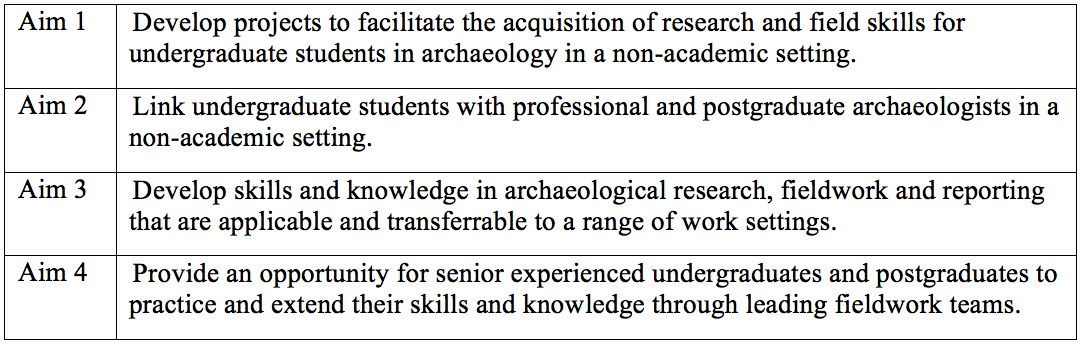
\includegraphics[width=\linewidth]{figures/Fyfe-Table01}
   		\captionof{table}{Aims of the non-academic skills development model.}
   		\centering
   		\label{fig:Fyfe-Table01}
   	\end{figure}	

   	\begin{figure} %TABLE 2
   		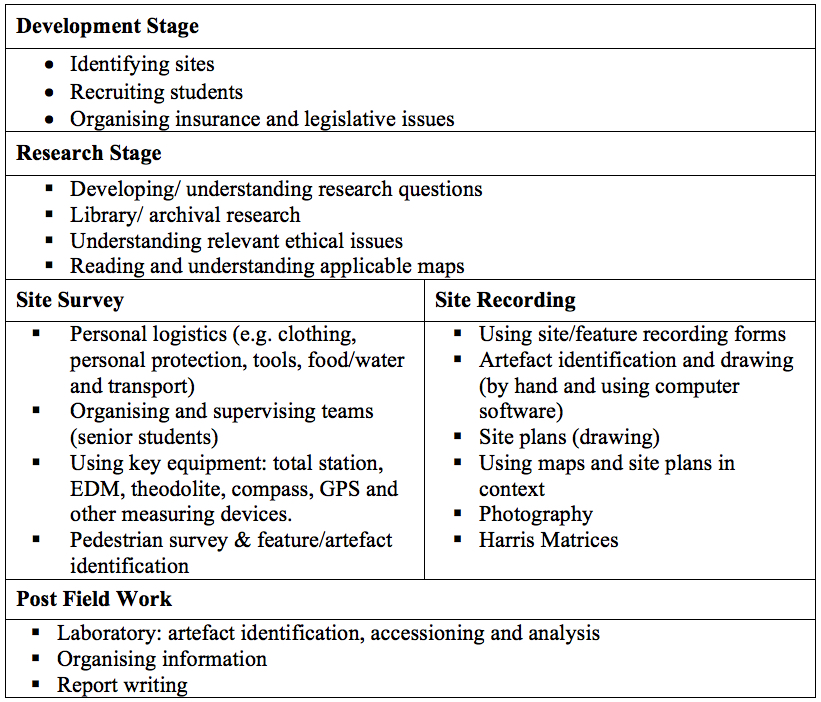
\includegraphics[width=\linewidth]{figures/Fyfe-Table02}
   		\captionof{table}{Aims of the non-academic skills development model.}
   		\centering
   		\label{fig:Fyfe-Table02}
   	\end{figure}

In addition, a template was created to give students a clear framework for planning and organising the research, gathering data and reporting it in an appropriate format. 
The final report format forms an important component of the archaeological record for sites for which little information is available, and contributes to the heritage of Western Australia in keeping with professional standards (e.g. \emph{Australian Archaeological Association, Australian Association of Consulting Archaeologists, World Archaeological Congress, and Society of American Archaeology Codes of Ethics}). 
The recording and reporting gives students a tangible outcome from the fieldwork, which \textcite[113-116]{mytum2012c} concludes is an important element of effective learning.

The first two stages allow for small groups, or individuals, to undertake desktop and archival research in preparation for the fieldwork component of the project. 
This develops and enhances research skills, implicit and explicit in project aims one and three. Similarly, maps accessed for the report, the results of background research and liaison with professional archaeologists, historians, librarians and others links to project aims one to three. 
The other stages allow for the incorporation of the data gathered in the field, including drawings and measurements, and relate well to the application of skills in aim three.

The model, with the identified skills and the reporting template, have been designed to meet the needs that students themselves identified, and to complement the skills developed through university courses in Australia \parencite[3]{beck2008}. 
The most likely employment for Australian graduates is to work in an archaeological consultancy, and the skill sets developed will be relevant to future careers in this area \parencites[e.g.][]{ireland2013}{ulm2005}{ulm2013}. 
There is also a degree of crossover with the academic side of the profession, where a similar set of research, technical and operational skills are important constituents of academic research.

\section{Case Study One: Canning Mills}

The first site for fieldwork was at Canning Mills, located on the outskirts of the Perth metropolitan area, approximately \SI {30}{\kilo\meter} 
to the south east of the city centre (\cref{fig:Fyfe-Figure01}). 
The site is an abandoned timber mill with an adjacent residential area, in use between c.1890 and 1930. 
Much of the land was rehabilitated, and has returned to forest, but a number of features are still visible. The site is not registered or protected under any legislative or regulatory provisions; it is in a semi-remote location on public land, and there is rapid degradation from large scale rubbish dumping and bushfires. A number of archaeological features (including structural foundations) are extant and, with easy access from the city, it was an ideal location to test the model.

   	\begin{figure} %FIGURE 1
   		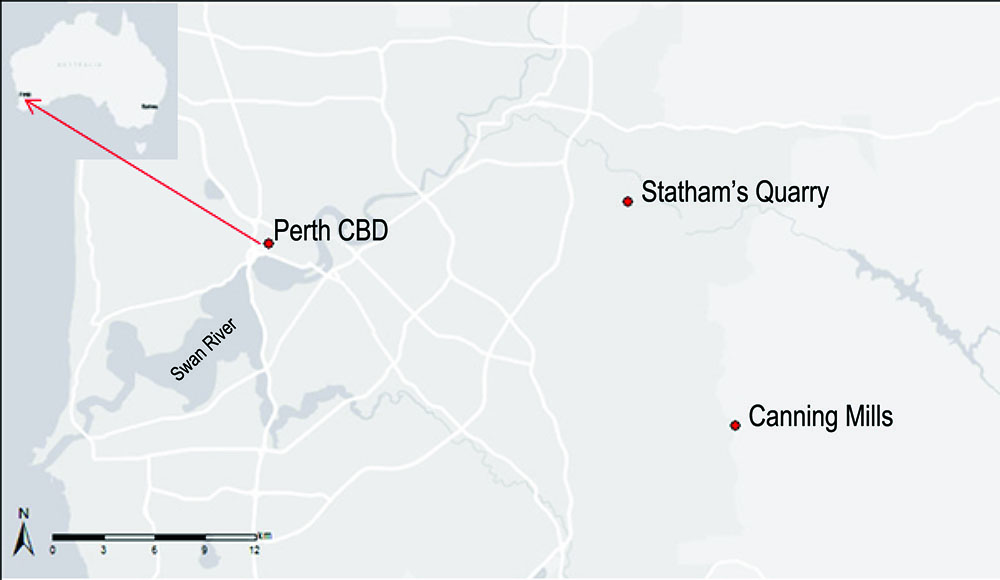
\includegraphics[width=\linewidth]{figures/Fyfe-Figure01}
   		\caption{Map showing the location of the sites referred to in this study, Canning Mills and Statham’s Quarry.}
   		\centering
   		\label{fig:Fyfe-Figure01}
   	\end{figure}

ASWA used social media, lecture announcements and emails to alert students to this fieldwork opportunity, and provided public liability insurance cover for the member volunteers. 
Demand from members was so high that a cap was set on the numbers able to participate. 
This meant there were enough students and supervisors sufficient to form five teams, each of which would undertake specific aspects of site recording.

Fieldwork processes and the skills to be developed were framed around an appropriate research question, following the initial site inspection. A self-selected group undertook archival and library research, identifying and accessing maps and documents relevant to planning the fieldwork.
Fieldwork logistics were the responsibility of fieldwork leaders, and all participants were responsible for their own personal protective equipment and field equipment, including field books, food and water.

Professional archaeologists including PhD candidates, consultants and museum staff led fieldwork. 
The field day began with an occupational health and safety briefing, site background, team allocations and responsibilities. Two teams conducted pedestrian surveys. One survey used \SI{5}{\meter} transects of the revegetated bushland to identify and record surface scatters of artefacts and a fenced grave. 
One team surveyed the edge of the road bordering the site, locating and recording the remains of a rail line used for timber transport while another team recorded and photographed surface scatters of glass, ceramics and metal remains across the open area of the site to the south of the roadway. 
Background research and maps of the site suggested that there had been a cricket pitch with buildings to the south east, and a team searched in dense bush for remains of these structures, however failed to find any evidence, an important experience for the students. 
Finally, the fifth team drew a plan of the remains of a large house with an extant curved stairway at the entrance and substantial remains of the foundations.

During the field day students were involved in site survey, feature identification, artefact identification and drawing, photography, site drawing, using GPS to record and locate features, map reading, data recording and team work. 
Communication was an essential skill at this large, densely forested site where only two of the teams were within visual range of one another; team leaders and the site director ensured that each team was well-briefed and contactable, an important precaution and planning skill for archaeologists in Australia who often work in isolated areas. 
In addition, some senior students had an opportunity to lead teams, make interpretations and decisions in the field, to guide less experienced students.

\section{Evaluating the Process}

Feedback from participants on the field day was excellent, with most students indicating that they relished the opportunity to practice skills they had learnt, or been introduced to, at university. 
The documentation produced by the students also showed that it had been an effective learning experience, with usable data, plans, and a range of drawings and photographs documenting the site. 
Writing of the post-field report was problematic. Students self-selected to write the report, but with the return to university life, including assessments and exams, the report writing lingered and was gradually abandoned. It was eventually completed by one of the postgraduate supervisors with little input from other members post field day.

The evaluation was that preparation for fieldwork and participation may generate enthusiasm and excellent results in terms of skill development and application. 
A lack of supervision and/or personal incentive after the field day led to a waning of that passion, and the result was that analysis and reporting skills important to future archaeological work were not practiced.

The model was revised to include a different post-fieldwork reporting process. While a report may be the preferable outcome, any output that forms an accessible, permanent record of archaeological work at the site is acceptable. 
The revised model also allocated the reporting phase to a single student, mentored by a professional archaeologist, which meant that the report process was manageable and provided that student with an outcome that could be listed on their CV. 
In addition, this second version of the model allowed for a range of alternative measurable outcomes, such as posters, conference presentations or reflective essays, dependent upon the needs of the project and to the benefit of the particular student. 
This meant that individuals could use the project to contribute to their wider skills resume, improving motivation as well as knowledge and skills for employment (\cref{fig:Fyfe-Figure02}). This was also designed to be more flexible to respond to the differences in sites, the needs of individuals and to provide a range of measurable outcomes.

   	\begin{figure} %FIGURE 2
   		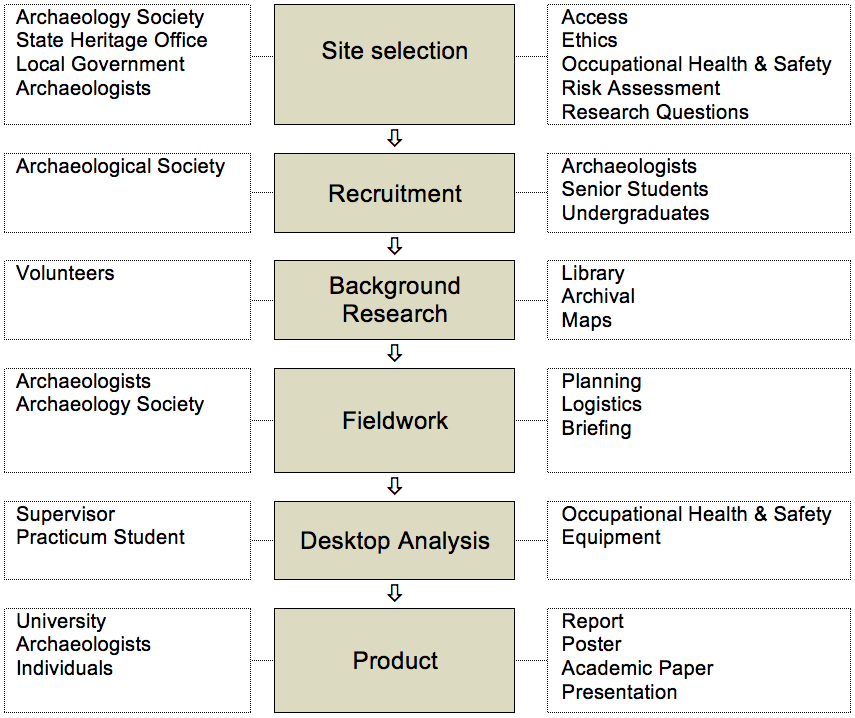
\includegraphics[width=\linewidth]{figures/Fyfe-Figure02}
   		\caption{Revised skills development model.}
   		\centering
   		\label{fig:Fyfe-Figure02}
   	\end{figure}

\section{Case Study Two: Statham's Quarry}

The revised model was used at Statham’s Quarry, a late 19th to early 20th century industrial complex located in the Darling Range east of Perth, Western Australia (\cref{fig:Fyfe-Figure01}). Unlike Canning Mills this site is listed on the State Heritage Register. It is located in Gooseberry Hill National Park and is a popular location for bushwalkers, rock climbers and a range of other recreational activities; therefore, access was not an issue.

Once again, there was high demand for this field day, and the 30 available positions filled within a few days. A team of five students conducted the archival research for the site before the field day, and 28 students, and four archaeologists, including one from the State Heritage Office, undertook the fieldwork. 
In a single day of survey, 46 archaeological features were recorded. 
Students gained valuable experience in research and site survey methodology (see \cref{fig:Fyfe-Figure03}), successfully gathering information on the layout and operation of the quarry, and associated industrial and residential buildings. 
The size of Statham’s Quarry allowed students to be involved in assessing multiple features at the site and to record them accurately under supervision. Therefore, students applied their skills using a variety of archaeological tools and methods likely to be utilised by companies in the professional sphere.

   	\begin{figure} %FIGURE 3
   		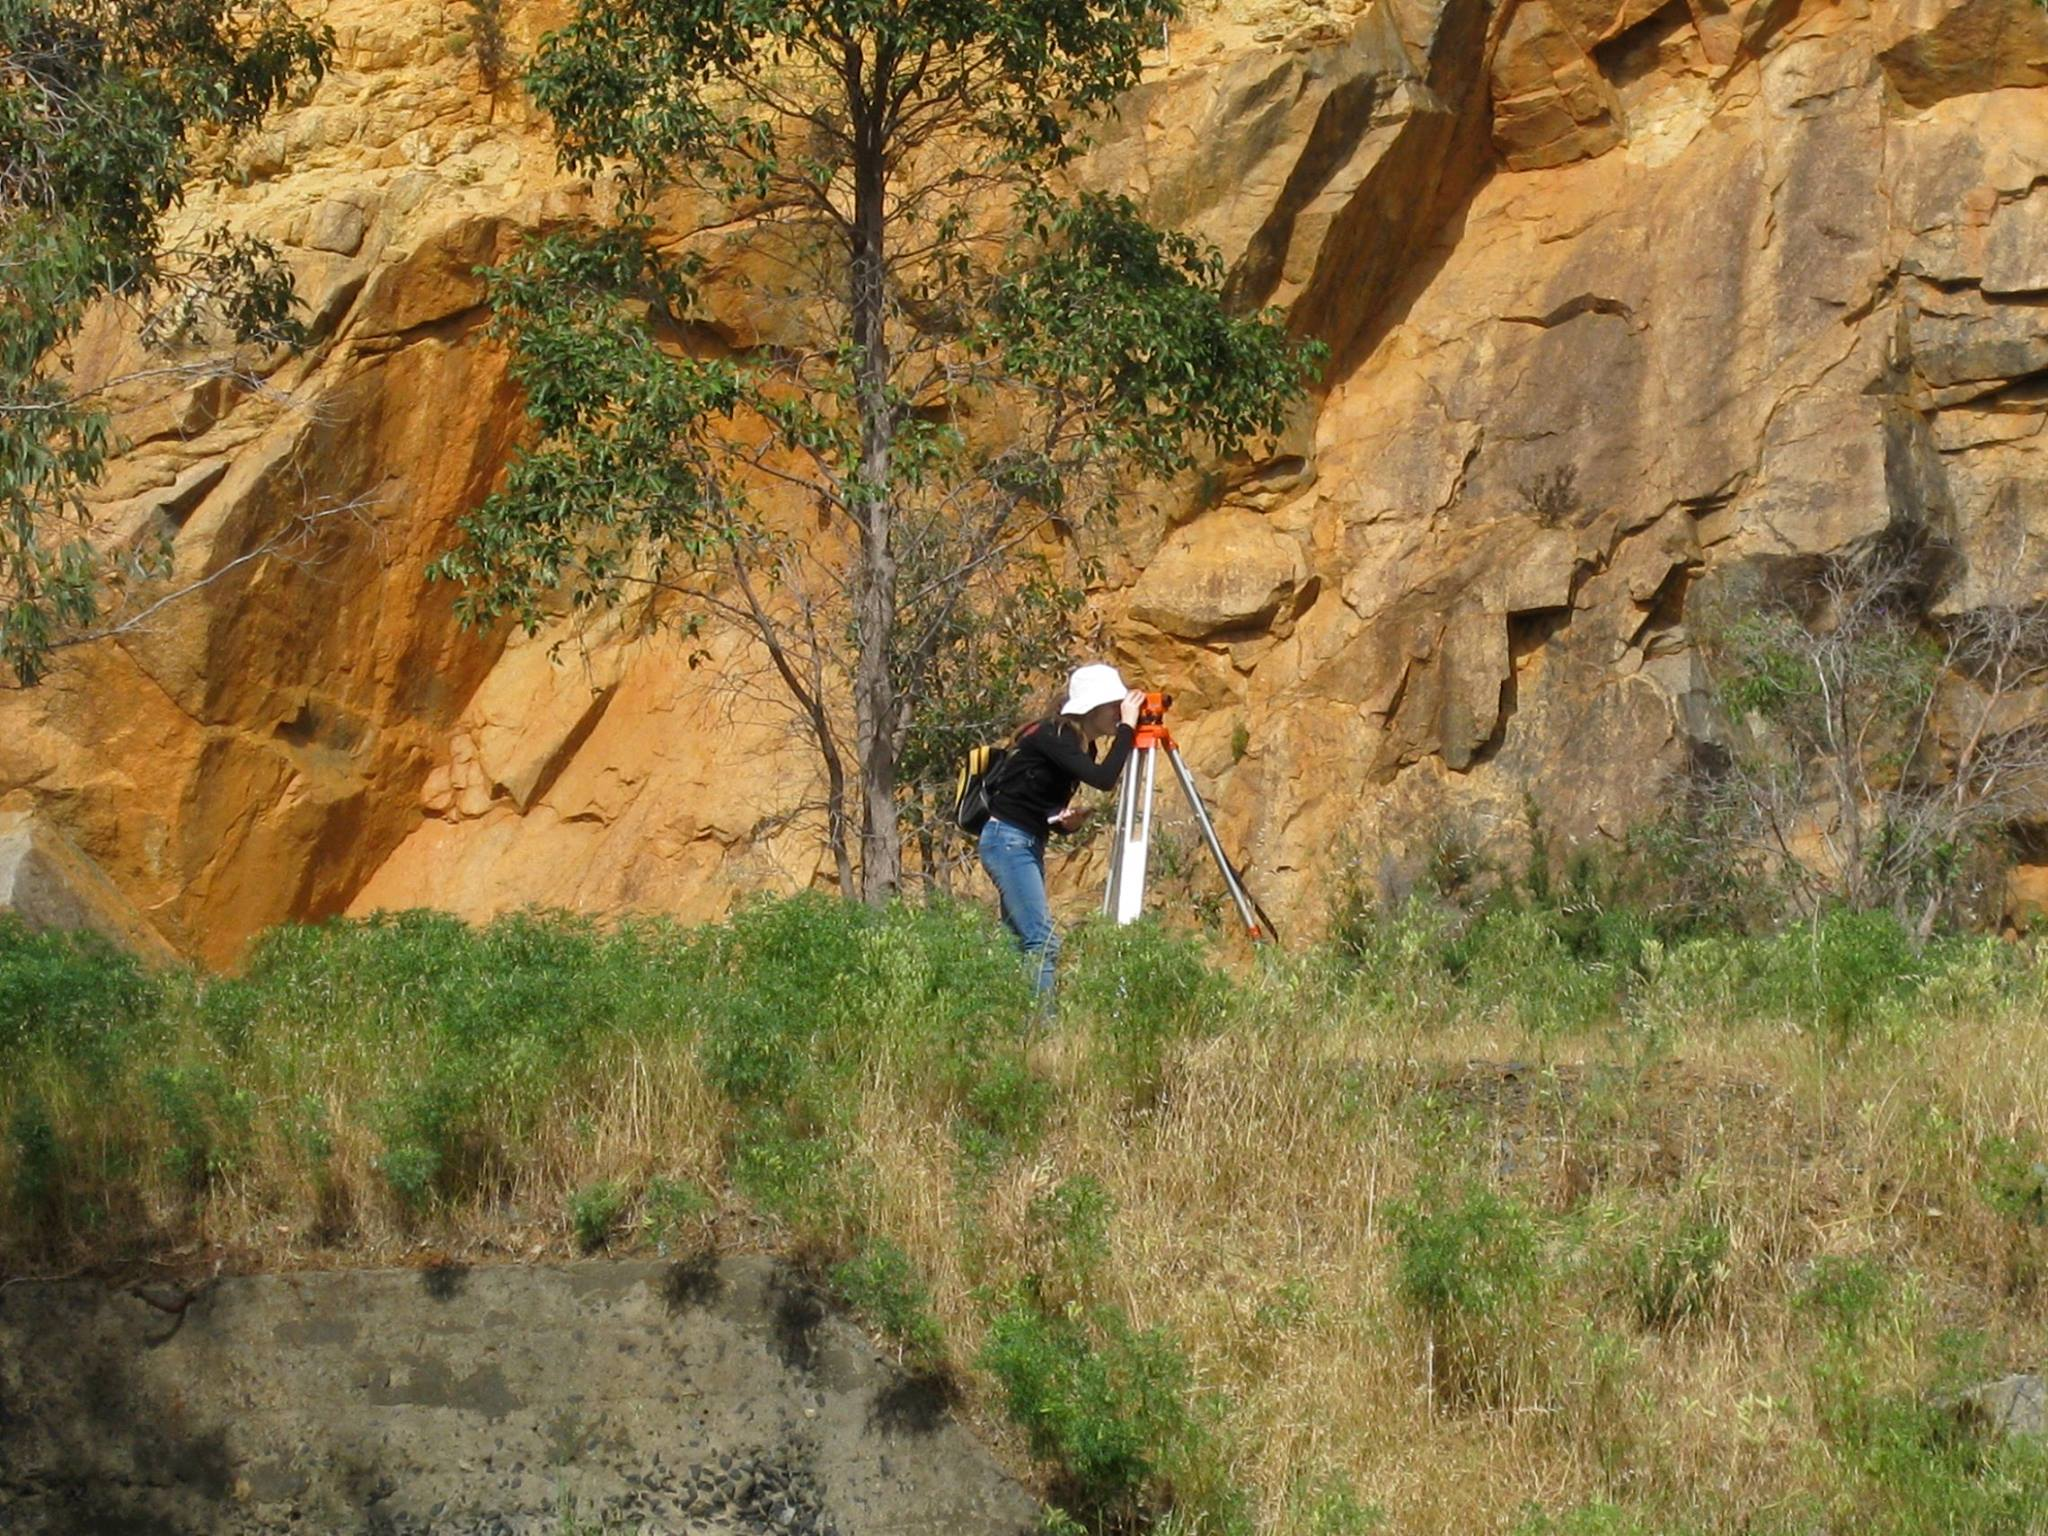
\includegraphics[width=\linewidth]{figures/Fyfe-Figure03}
   		\caption{Revised skills development model.}
   		\centering
   		\label{fig:Fyfe-Figure03}
   	\end{figure}

As planned, a report \parencite{murszewskiwinter2012} was produced by an undergraduate student overseen by a professional archaeologist, 
and a poster \parencite{murszewski2012} was also produced and displayed at the 2012 Australasian Institute for Maritime Archaeology (AIMA)/Australasian Society for Historical Archaeology (ASHA) Conference. 
The model was tested during a further small-scale survey of the Statham’s Quarry site, and used again in the following year in a small historic project for a private landowner, which also resulted in a conference poster \parencite{busher2012}, also for the 2012 AIMA/ASHA Conference.

The model demonstrated that it could provide experiential learning for a large number of students with a wide range of skills in research, fieldwork, analysis and reporting; all of which were applicable to their future employment as well as their current studies. 
With revisions, the model has demonstrated its value. The case studies and subsequent applications show that the model is flexible and responsive to student and community needs. 
Students are able to drive their own involvement in fieldwork, lessening their dependence upon being invited to participate in existing projects. Beyond this, the mentoring relationship between students and professionals allowed students exposure to a wider range of knowledge and experience than might otherwise have been the case.

\section{Discussion}

The need for practical skills in archaeology is essential \parencites{boytner2012}{cobb2012}{colley2012}{mytum2012a}{mytum2012b}{ulm2013} and the model described above is designed to allow students to develop those skills, within a workable, easy to organise, low cost, high participation framework. 
It is driven, not by a university derived curriculum framework, but by students seeking regular participatory access to field experiences. As such, the model may be considered a version of ‘archaeology from below’, a socialist archaeological approach articulated by \textcite{faulkner2000}, in which the participants (the students) are involved in all aspects of the project from design, through to fieldwork and reporting. 
Undergraduate students were, and continue to be, involved at all levels, from identification of the need, development of the project and recruitment of professional archaeologists, to background site research, some supervision and leadership during field days and subsequent report writing.

While overall background development of the projects and mentoring during field days is provided by professional qualified archaeologists, students participate in research design, and in articulating the skills they wish to develop. 
There is variation in the extent of participation by students, with some heavily involved in all aspects, while others limit their involvement to attendance at the field days. 
Typically, those students with an interest in pursuing archaeology as a career are most heavily involved, while those with a more casual interest in the discipline have less investment in the projects. The flexibility of the model allows those varied levels of involvement. The participation of professional archaeologists is similarly variable. 
Qualified archaeologists from a range of backgrounds were approached to provide their time and expertise as volunteers, and people from academia, commercial archaeology, and regulatory bodies, as well as industry and museum departments, volunteered to assist with field days. 
Students were consequently exposed to numerous qualified archaeologists with a range of experience, and this is considered one of the successes of the model. Through this process, the students gained exposure to a range of professional skills and opinions, gaining a wider understanding of approaches to site recording. 
Enterprising students were also able to meet professionals from backgrounds beyond those normally encountered in academia, and to impress potential future employers. 
The success of this exposure to archaeologists from outside academia led ASWA to develop an annual event, dubbed ‘Archy-Con’, inviting archaeologists from a range of backgrounds in Western Australia to meet and share their experiences with students.

The other success of the model is its emphasis on unregistered, often at risk, sites, located on public land. This approach allows the recording of baseline data for sites at risk of immediate destruction. While not considered highly significant, these sites still have the potential to provide useful data to future researchers. 
Significance is a mutable quality \parencites{bowdler1984}{brown2008} and while these sites may not be considered significant now, that may change in future, and this baseline recording provides a heritage service to the Community and the state of Western Australia. 

The insistence that projects be student driven from start to finish, develops an understanding of why archaeology is conducted, as well as how, and emphasises the necessity to practice archaeology within a consistent ethical framework and with a research outcome in mind, rather than simply for the sake of it. 
Fieldwork is configured as the data-gathering phase of a larger archaeological process based on research questions, rather than conducted for its own sake. 

The final phase of the model, post-fieldwork report writing, proved to be one of the less successful aspects. When questioned students suggested they were comfortable conducting background research and fieldwork under supervision, but were much less comfortable writing within the framework of a report. 
This may have been due to unfamiliarity with the format, or the fact that writing their results was more time consuming than other aspects of the project. Regardless, without providing an incentive to do them, reports (or other appropriate outputs) would not have been produced.

From the beginning, the model was developed for best practice in historical archaeology, much of which, in terms of the documentation and recording processes, can be translated to other sub-disciplines within archaeology. 
The general framework of the model of student driven participation in research and fieldwork has been successfully adapted to a number of projects. These include contemporary archaeology projects recording a threatened beach community dating to the 1960's, or recording graffiti in the city of Perth, and a maritime archaeology project recording a shipwreck in shallow water in the Swan River. 
Laboratory projects have also been conducted using this model, with students successfully taking control of, and running, the accessioning and analysis of a number of large artefact assemblages. This has resulted in a range of outputs such as databases, reports, conference posters, submissions to existing heritage registers and artefact catalogues. 
Two papers are also currently in preparation for publication in peer reviewed journals. All of the outputs were produced wholly, or with substantial input, from the student members of ASWA.

One Australian archaeology sub-discipline where the model has not yet been used is Indigenous archaeology. The ethical and regulatory issues associated with working on Indigenous sites in Australia requires a greater level of consultation than those of non-Indigenous sites and these may be better dealt with within the more structured framework of academic and/or consultancy research. 
While the model could be applied to Indigenous sites, a greater degree of planning and consultation, and a multi-year time frame, would be required to meet regulatory requirements and ethical standards.

One difficulty encountered with the model was continuity within ASWA itself. Most students are members for no more than three years and members of the Executive are usually in their positions for only one year, meaning the window for passing on the operation of the model is brief. 
ASWA developed a position within the Executive responsible for liaison with qualified archaeologists in order to continue the organisation of field days; however, the ongoing success of the model has been dependent upon the energy of the office holder. 
Fortunately, longer term postgraduate members of ASWA have allowed a level of knowledge transfer and continuity in the development and application of the model.

\section{Conclusion}

The innovative and structured approach developed by the Archaeological Society of Western Australia and described in this paper, has shown how a flexible approach is essential for a non-academic model, to allow it to be applied to a variety of projects, whilst meeting both the ethical and legal needs consistent with good archaeological practice. 
The model offers real, tangible experiences to students to enhance their skills development and indeed, is driven by the desires and requirements of those students. This project was never intended to replicate or replace highly structured university based practical training; instead, it is designed to allow students to practice skills gained within that structured learning environment. 
The model allows students to initiate and be involved in projects from start to finish, and to tailor their involvement to their level of interest. Despite being tailored to Western Australian conditions, ASWA has developed a model that is flexible and responsive, not restricted by specific legislative requirements. 
It has the potential to be applied wherever there is a strong and motivated student body, professional archaeologists willing to volunteer their time, and sites which are low risk, low significance, accessible, affordable and able to be recorded with minimal impact, and maximum benefit. 

\section{Acknowledgements}

The Discipline of Archaeology at University of Western Australia for the equipment, facilities and laboratory space, and to Jane Balme for feedback on this paper. Thanks to the archaeologists who provided their services as supervisors during field days including Kelly Fleming, State Heritage Office, WA, Alice Beale, WA Museum, Renee Gardiner of Earth Imprints Consulting, Karina Williams of Eureka Archaeological Research and Consulting, Bob Sheppard of Heritage Detection Australia and Stafford Smith. Sarah Knight Regional Program Director ABC Radio for fieldwork and media coverage. Field day volunteers at Canning Mills, and Statham’s Quarry: John Adeney, Samara Allen, Sarah Ames, Natasha Busher, Nina Conway, Lauren Davidson, Matt Dix, Christa Entwhistle, Aaron Floky, Jonathan Gimblett, Alyce Haast, Lisa Hewson, Philipa Hudson, Victoria Kelly, Jess Laurier, Arianne Maggio, Erin Mein, Janet Osborne, Jannie Peircy, Emily Purvis, Malati Redeckis, Rebecca Ryan, Godfrey Rule, Zack Sheppard, Danielle Tassone, Katrina West and Gemma Wilson.

Special thanks to the dedicated and enthusiastic Executive Committees of the Archaeological Society of Western Australia who started this project and have maintained it from 2010 to the present.


\clearpage
\IJSRAclosing
\end{document}